\section{Math 202A - HW8 - Dan Davison - \texttt{ddavison@berkeley.edu}}

% 7.17. You're on the right track but are missing a lot of details. You need to justify commuting the integral and the limit (dominated convergence??). I don't know where you were going with your m's and delta's either. (-5)
% Aidan Backus, Nov 3 at 3:54pm
% 7.9. This problem doesn't count towards your grade but it's good that you're thinking of a Fatou lemma for limsups. In fact, if f_n is *nonpositive* on a measurable set A, then \limsup_n \int_A f \leq \int_A \limsup_n f_n; you can prove this by just multiplying everything in Fatou's lemma by -1's and noting that when you commute a -1 with a liminf it turns into a limsup.
% Aidan Backus, Nov 3 at 3:56pm
% 7.11. Your argument can be patched to work but it is false that F is an increasing function; what if f = sin? (-3)
% Aidan Backus, Nov 4 at 8:37am
% 4. Your g(x) is not integrable, so you cannot apply DCT. The dominating function you should try would bound (1+x/n)^-n by exp(-x/2), or something similar. This "slows down" the decay of g(x) enough to be dominating, but without introducing a constant that makes g non-integrable. (-7)
% Ian Francis, Nov 24 at 1:01am
% 7.11) 7 7.13) 3 7.17) 5 7.21) 10
% Ian Francis, Nov 24 at 1:01am


\begin{comment}
  \begin{mdframed}
    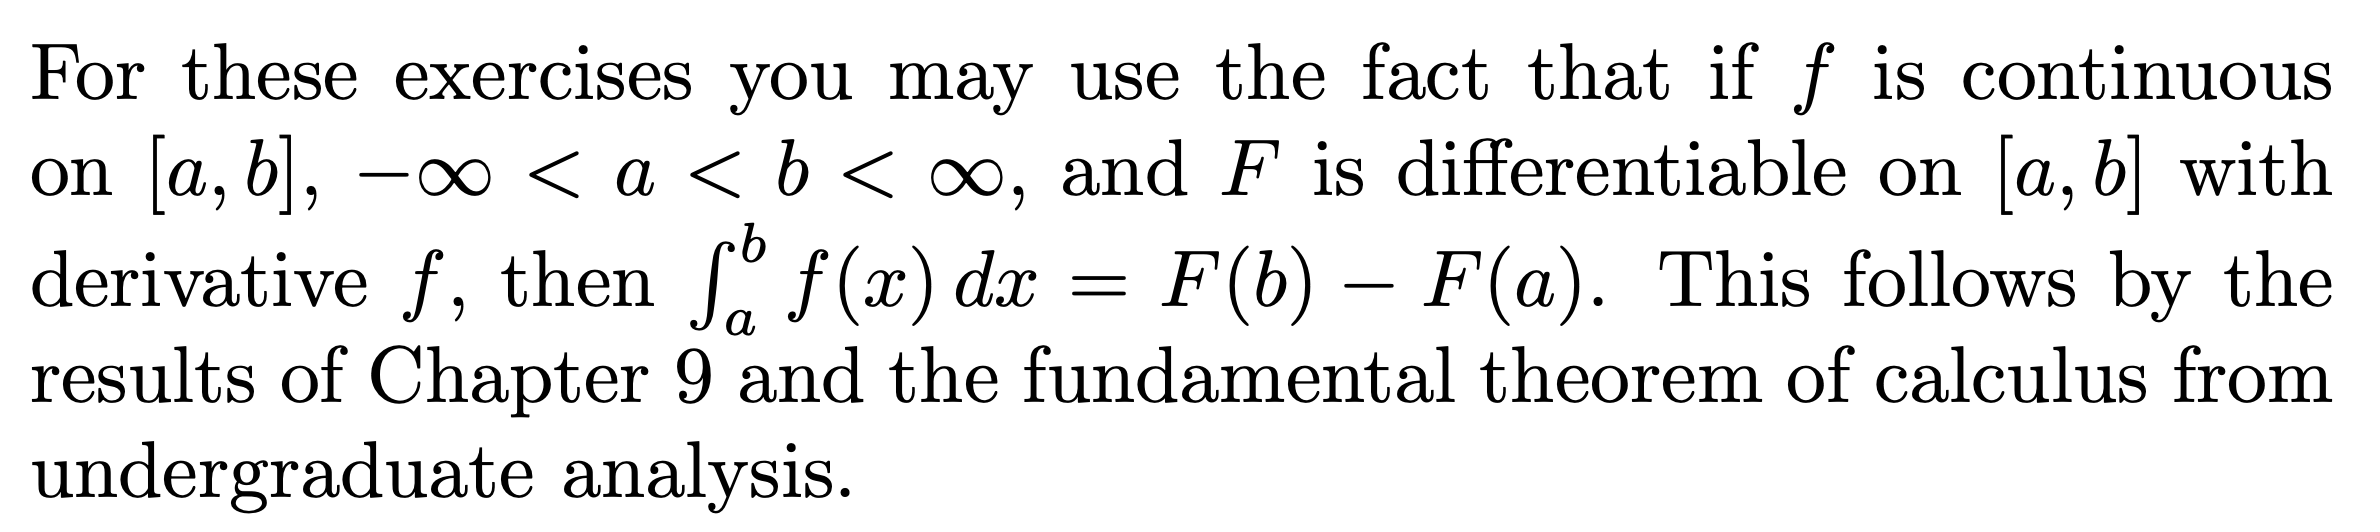
\includegraphics[width=400pt]{img/analysis--berkeley-202a-hw08-518d.png}
  \end{mdframed}
\end{comment}

\begin{mdframed}
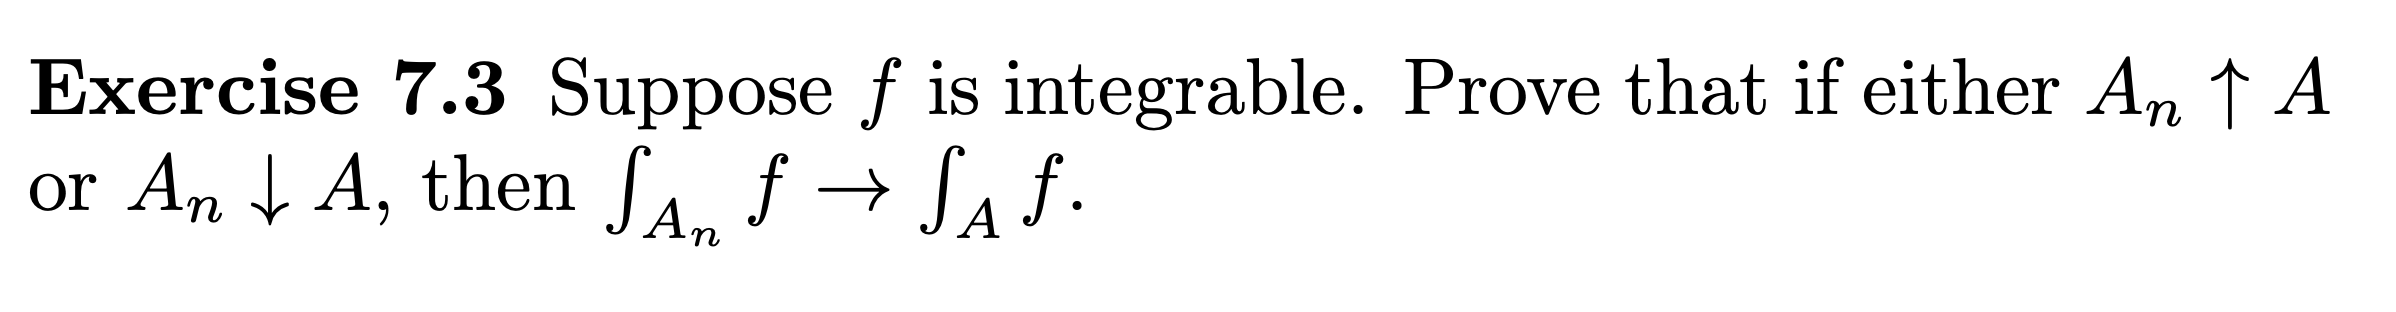
\includegraphics[width=400pt]{img/analysis--berkeley-202a-hw08-2798.png}
\end{mdframed}

\begin{proof}
  The required result is equivalent to
  \begin{align*}
    \limn \int f \ind_{A_n} = \int f \ind_A.
  \end{align*}

  Suppose first that $A_n \uparrow A$.

  Note that
  \begin{align*}
    \limn f\ind_{A_n} = f\limn\ind_{A_n} = f\ind_A,
  \end{align*}
  and furthermore that $|f\ind_{A_n}| \leq f$ for all $n$ and $f$ is integrable. Therefore by the dominated
  convergence theorem we have
  \begin{align*}
    \limn \int f \ind_{A_n} = \int f \ind_A,
  \end{align*}
  as required.

  Next suppose that $A_n \downarrow A$. Thus $A_n \supseteq A$ for all $n$, and $A_n^c \uparrow A^c$. In
  parallel with the previous argument we have
  \begin{align*}
    \limn f\ind_{A_n^c} = f\limn\ind_{A_n^c} = f\ind_{A^c},
  \end{align*}
  and furthermore $|f\ind_{A_n^c}| \leq f$ for all $n$ and $f$ is integrable.  Therefore by the dominated
  convergence theorem we have
  \begin{align*}
    \limn \int f \ind_{A_n^c} = \int f \ind_{A^c}.
  \end{align*}
  This can be written in terms of integrals over the original (non-complemented) sets as
  \begin{align*}
    \limn \Bigg(\int f - \int f \ind_{A_n}\Bigg) = \int f - \int f \ind_{A},
  \end{align*}
  or equivalently
  \begin{align*}
    \int f - \limn \int f \ind_{A_n} = \int f - \int f \ind_{A}.
  \end{align*}
  Since $\int f < \infty$ we may subtract $\int f$ from both sides, and then multiply by $-1$, yielding
  \begin{align*}
    \limn \int f \ind_{A_n} = \int f \ind_{A},
  \end{align*}
  as required.
\end{proof}

\newpage
\begin{mdframed}
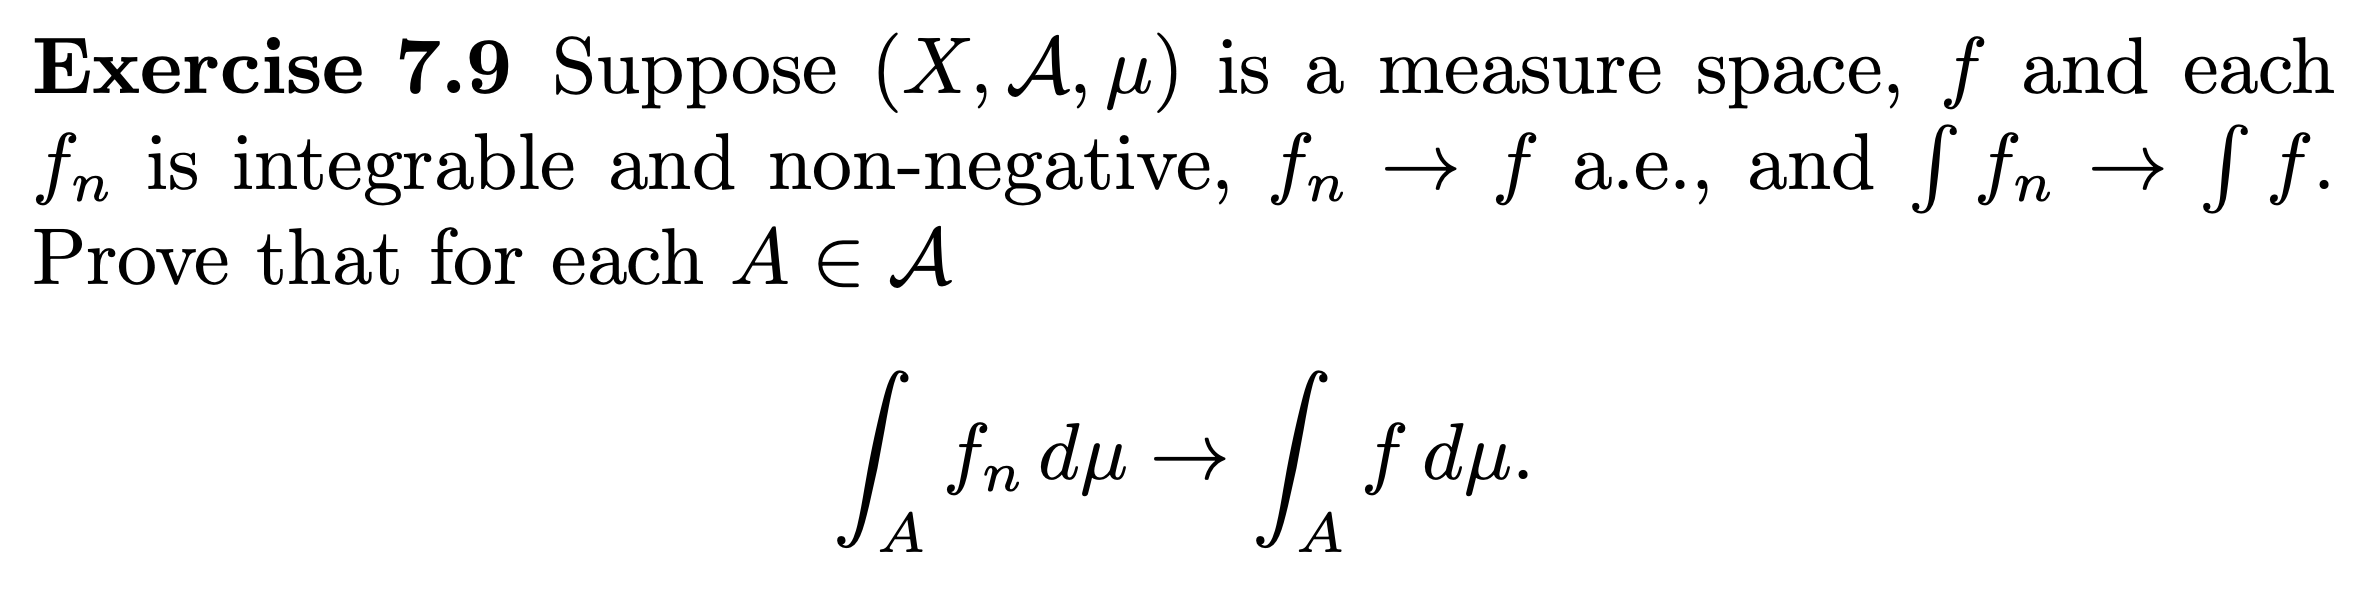
\includegraphics[width=400pt]{img/analysis--berkeley-202a-hw08-3203.png}
\end{mdframed}

% 7.9. This problem doesn't count towards your grade but it's good that you're thinking of a Fatou lemma for
% limsups. In fact, if f_n is *nonpositive* on a measurable set A,
% then $\limsup_n \int_A f \leq \int_A \limsup_n$ f_n; you can prove this by just multiplying everything in
% Fatou's lemma by -1's and noting that when you commute a -1 with a liminf it turns into a limsup.

% Aidan Backus , Nov 3 at 3:56pm


\begin{comment}
  \begin{remark*}
    We have that $\int_X f_n \to \int_X f$. What we must show is that this limit-of-integrals still holds when
    the integrals are restricted to $A \subset X$.

    In general, this is not true. For example, let $X = [0, 1]$ and let $f(x) = 0$. Now for odd $n$, let $f_n(x)$
    take the value $-1$ for $0 \leq x < 0.5$ and $+1$ for $0.5 \leq x \leq 1$, and for even $n$ let it take $+1$
    on the first interval and $-1$ on the second. Then $\int_X f_n = 0 = \int_X f$ for all $n$, so the
    hypothesis $\int_X f_n \to \int_X f$ does hold. But $\int_{[0, 0.5]} f_n$ is the
    sequence $-\frac{1}{2}, +\frac{1}{2}, -\frac{1}{2}, \ldots$ and thus has no limit.

    What we need to show is that the result does hold with the additional hypotheses.
  \end{remark*}

\end{comment}
\begin{proof}
  Note that $\int_A f_n = \int f_n\ind_A$ and that $f_n\ind_A \to f\ind_A$ a.e. Therefore by Fatou's lemma we have
  \begin{align*}
    \liminfn \int_A f_n \geq \int_A f.
  \end{align*}
  Now, we would like to show that
  \begin{align}
    \limsupn \int_A f_n \leq \int_A f.
  \end{align}
  since then we would have
  \begin{align*}
    \int_A f \leq \liminfn \int_A f_n \leq \limsupn \int_A f_n \leq \int_A f,
  \end{align*}
  which implies that
  \begin{align*}
    \limn \int_A f_n = \int f,
  \end{align*}
  as required.

  However, I'm not sure how to show (1). It's tempting to think that it's a theorem that always holds -- i.e. a
  counterpart to Fatou's lemma. But, there are counterexamples, such as $f_n = \ind_{[n, n+1]}$.

  What have we made use of?
\begin{verbatim}
  |-------------------------+-------------|
  | non-negativity of f_n   | yes - Fatou |
  | convergence of f_n a.e. | yes         |
  | non-negativity of f     | no          |
  | integrability of f      | no          |
  | integrability of f_n    | no          |
  | convergence of int f_n  | no          |
\end{verbatim}
\end{proof}


\newpage
\begin{mdframed}
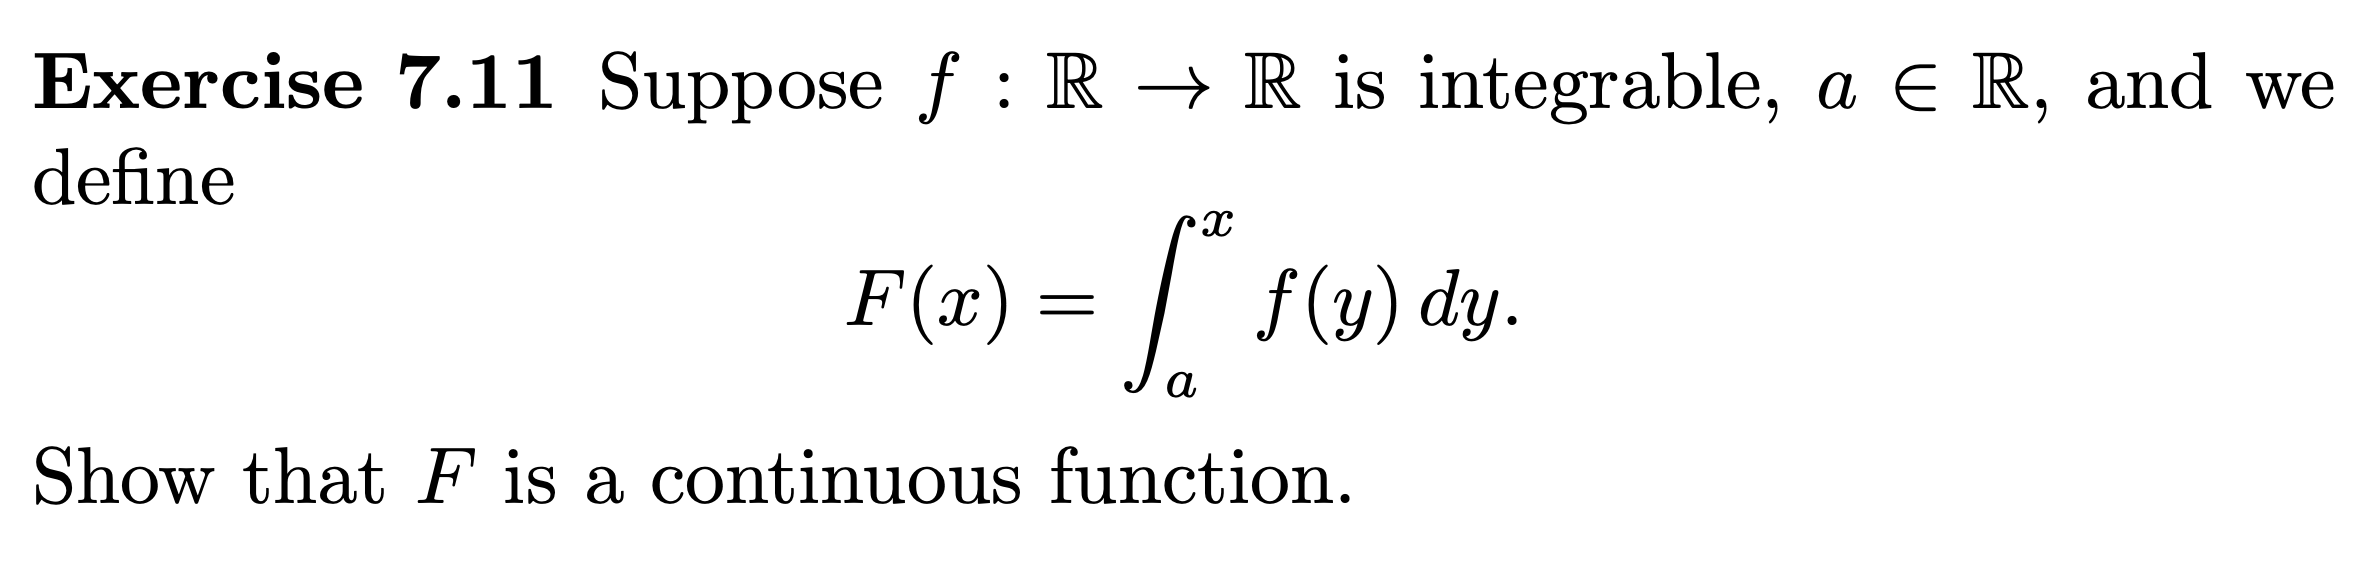
\includegraphics[width=400pt]{img/analysis--berkeley-202a-hw08-d0c0.png}
\end{mdframed}

% 7.11. Your argument can be patched to work but it is false that F is an increasing function; what if f = sin? (-3)

\begin{comment}
  \begin{intuition*}
    $F$ is an increasing function $\R \to \R$. To say that it is continuous is to say that a small extension to
    the interval being integrated over results in a small extension to the area. This implies that there is
    some limit to how much area is added by a small interval $[b, b + \delta]$.
  \end{intuition*}
\end{comment}

\begin{proof}
  Let $\eps > 0$ and let $b \in \R$.

  We must show that there exists $\delta > 0$ such that if $x \in \(b - \delta, b + \delta\)$
  then $F(x) \in \(F(b) - \eps, F(b) + \eps\)$.

  Note that $F$ is an increasing function, therefore it suffices to show that there exists $\delta$ such
  that $F(b - \delta) > F(b) - \eps$ and $F(b + \delta) < F(b) + \eps$.

  First we will show that there exists $\delta > 0$ such that $F(b + \delta) < F(b) + \eps$. Note that
  \begin{align*}
    F(b + \delta) := \int_{[a, b + \delta]} f = F(b) + \int_{[b, b + \delta]} f,
  \end{align*}
  therefore it suffices to show that there exists $\delta > 0$ such that $\int_{[b, b + \delta]} f < \eps$.
  This follows from HW7 Bass Ex. 6.4.

  Secondly we will show that there exists $\delta > 0$ such that $F(b - \delta) > F(b) - \eps$. Note that
  \begin{align*}
    F(b) = F(b - \delta) + \int_{[b - \delta, b]} f,
  \end{align*}
  hence
  \begin{align*}
    F(b - \delta) = F(b) - \int_{[b - \delta, b]} f,
  \end{align*}
  therefore it suffices to show that there exists $\delta > 0$ such that $\int_{[b - \delta, b]} f < \eps$.
  Again, this follows from HW7 Bass Ex. 6.4.
\end{proof}

\newpage
\begin{mdframed}
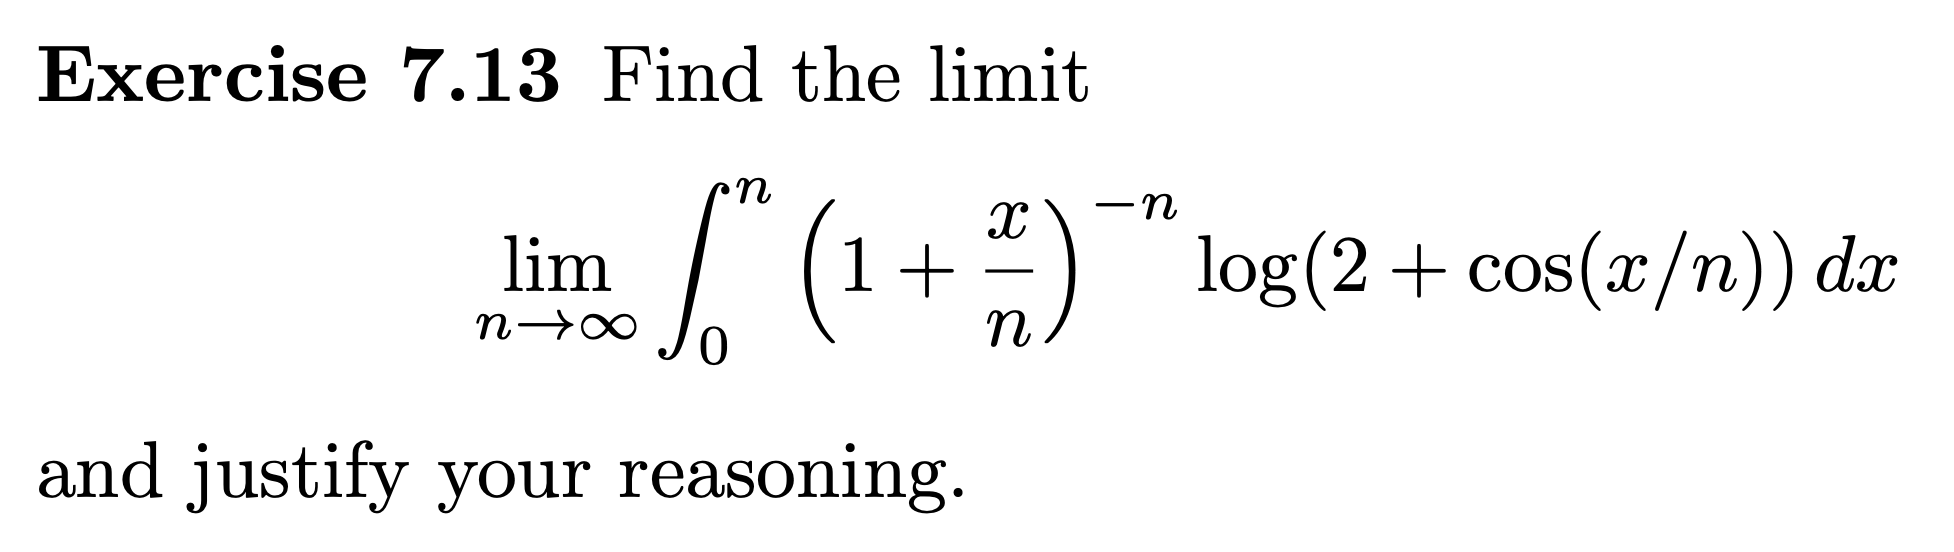
\includegraphics[width=400pt]{img/analysis--berkeley-202a-hw08-9931.png}
\end{mdframed}

% 4. Your g(x) is not integrable, so you cannot apply DCT. The dominating function you should try would bound
% (1+x/n)^-n by exp(-x/2), or something similar. This "slows down" the decay of g(x) enough to be dominating,
% but without introducing a constant that makes g non-integrable. (-7)

\begin{proof}
  Let $f(n) = (1 + x/n)^{-n} \log(2 + \cos(x/n))$.

  Note that $2 + \cos(x/n) \geq 1$ and therefore that $f_n\ind_{[0, n]} \geq 0$ for all $n$.

  Note also that $f(n)\ind_{[0, n]}$ is bounded above by $g(x) = \frac{\log 3}{1 + x}$.

  Therefore
  \begin{align*}
    \limn \int_0^n f_n
    &:=\limn \int f_n\ind_{(0, n)}                                        \\
    &= \int \limn f_n\ind_{(0, n)}                                        ~~~~~~~ \text{(by the dominated convergence theorem)}\\
    &:= \int \limn (1 + x/n)^{-n} \log(2 + \cos(x/n))\ind_{(0, n)}(x)\dx  \\
    &= \log 3\int_0^\infty e^{-x} \dx                                     ~~~~~~~ \text{(by Bass prop 6.3 (c) regarding pulling a constant out of integral})\\
%    &= -\log 3 [e^{-x}]_0^\infty \\
    &= \log 3.                                                           ~~~~~~~  \text{(by note provided with ch 7. exercises regarding use of antiderivative to evaluate integral)}
  \end{align*}

\end{proof}

\newpage
\begin{mdframed}
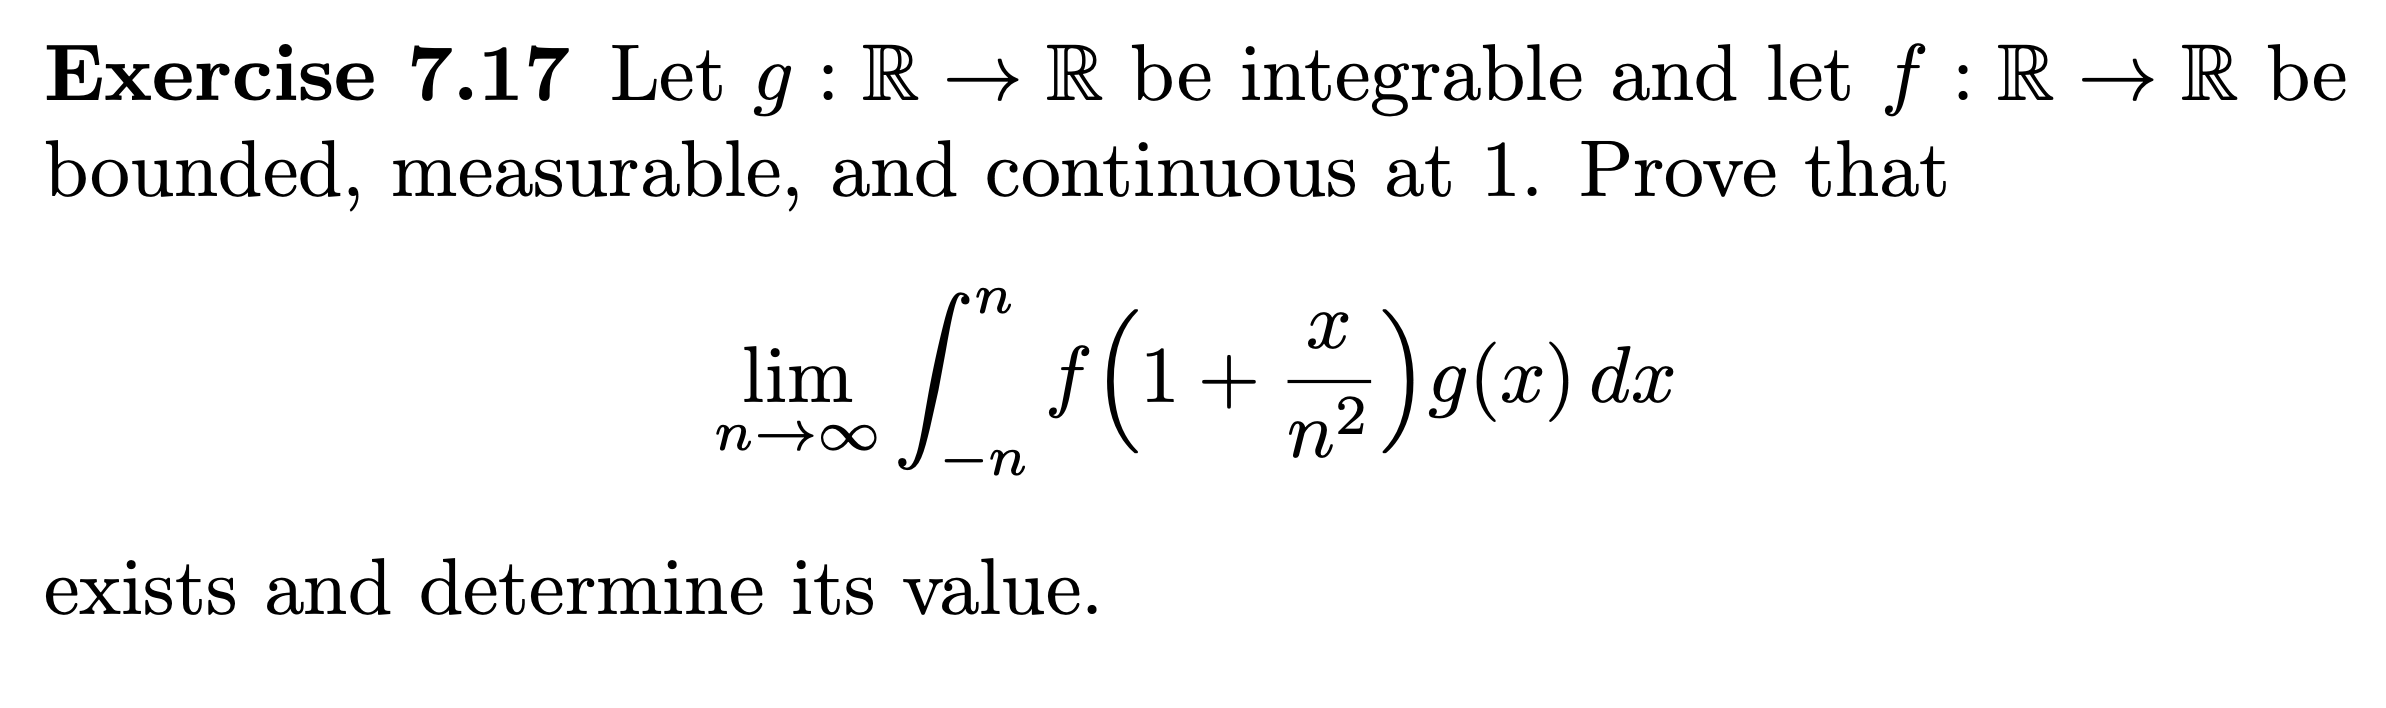
\includegraphics[width=400pt]{img/analysis--berkeley-202a-hw08-6e60.png}
\end{mdframed}

% 7.17. You're on the right track but are missing a lot of details. You need to justify commuting the integral
% and the limit (dominated convergence??). I don't know where you were going with your m's and delta's either.
% (-5)

% Aidan Backus , Nov 3 at 3:54pm


\begin{remark*}
  The integrand may be unbounded. For example, take $g(x) = |x|^{-1/2}$ and $f = 1$. Then the integrand is
  equal to $g$ and is integrable and unbounded.
\end{remark*}

\begin{proof}
    Let $\eps > 0$.

    Since $f$ is continuous at $1$ there exists $\delta > 0$ such that if $y \in (1 - \delta, 1 + \delta)$
    then $f(y) \in (f(1) - \eps, f(1) + \eps)$.

    Fix $m \in \N$ such that $1/m < \delta$.

    Note that for $n \geq m$ we have that if $x \in (-n, n)$
    then
    \begin{align*}
      1 + \frac{x}{n^2} \in \Big(1 - \frac{1}{n}, 1 + \frac{1}{n}\Big) \subseteq (1 - \delta, 1 + \delta),
    \end{align*}
    and therefore
    \begin{align*}
      f\Big(1 + \frac{x}{n^2}\Big) \in \big(f(1) - \eps, f(1) + \eps\big).
    \end{align*}

    Let $h_n(x) = f(1 +\frac{x}{n^{2}})g(x)$.

    Then for $n \geq m$ and $x \in (-n, n)$ we have
    \begin{align*}
      h_n(x) \in \Big((f(1) - \eps)g(x), (f(1) + \eps)g(x)\Big).
    \end{align*}
    Since $\eps > 0$ is arbitrary, we have that $h_n \to f(1)g$ pointwise.

    We must prove that $\limn \int h_n \ind_{(-n, n)}$ exists and determine its value.

    We have (\red{TODO} make this argument solid)
    \begin{align*}
      \limn \int h_n \ind_{(-n, n)}
      &= \lim_{n \geq m} \int h_n \ind_{(-n, n)} \\
      &= f(1)\int_{-\infty}^\infty g.
    \end{align*}
\end{proof}

\newpage
\begin{mdframed}
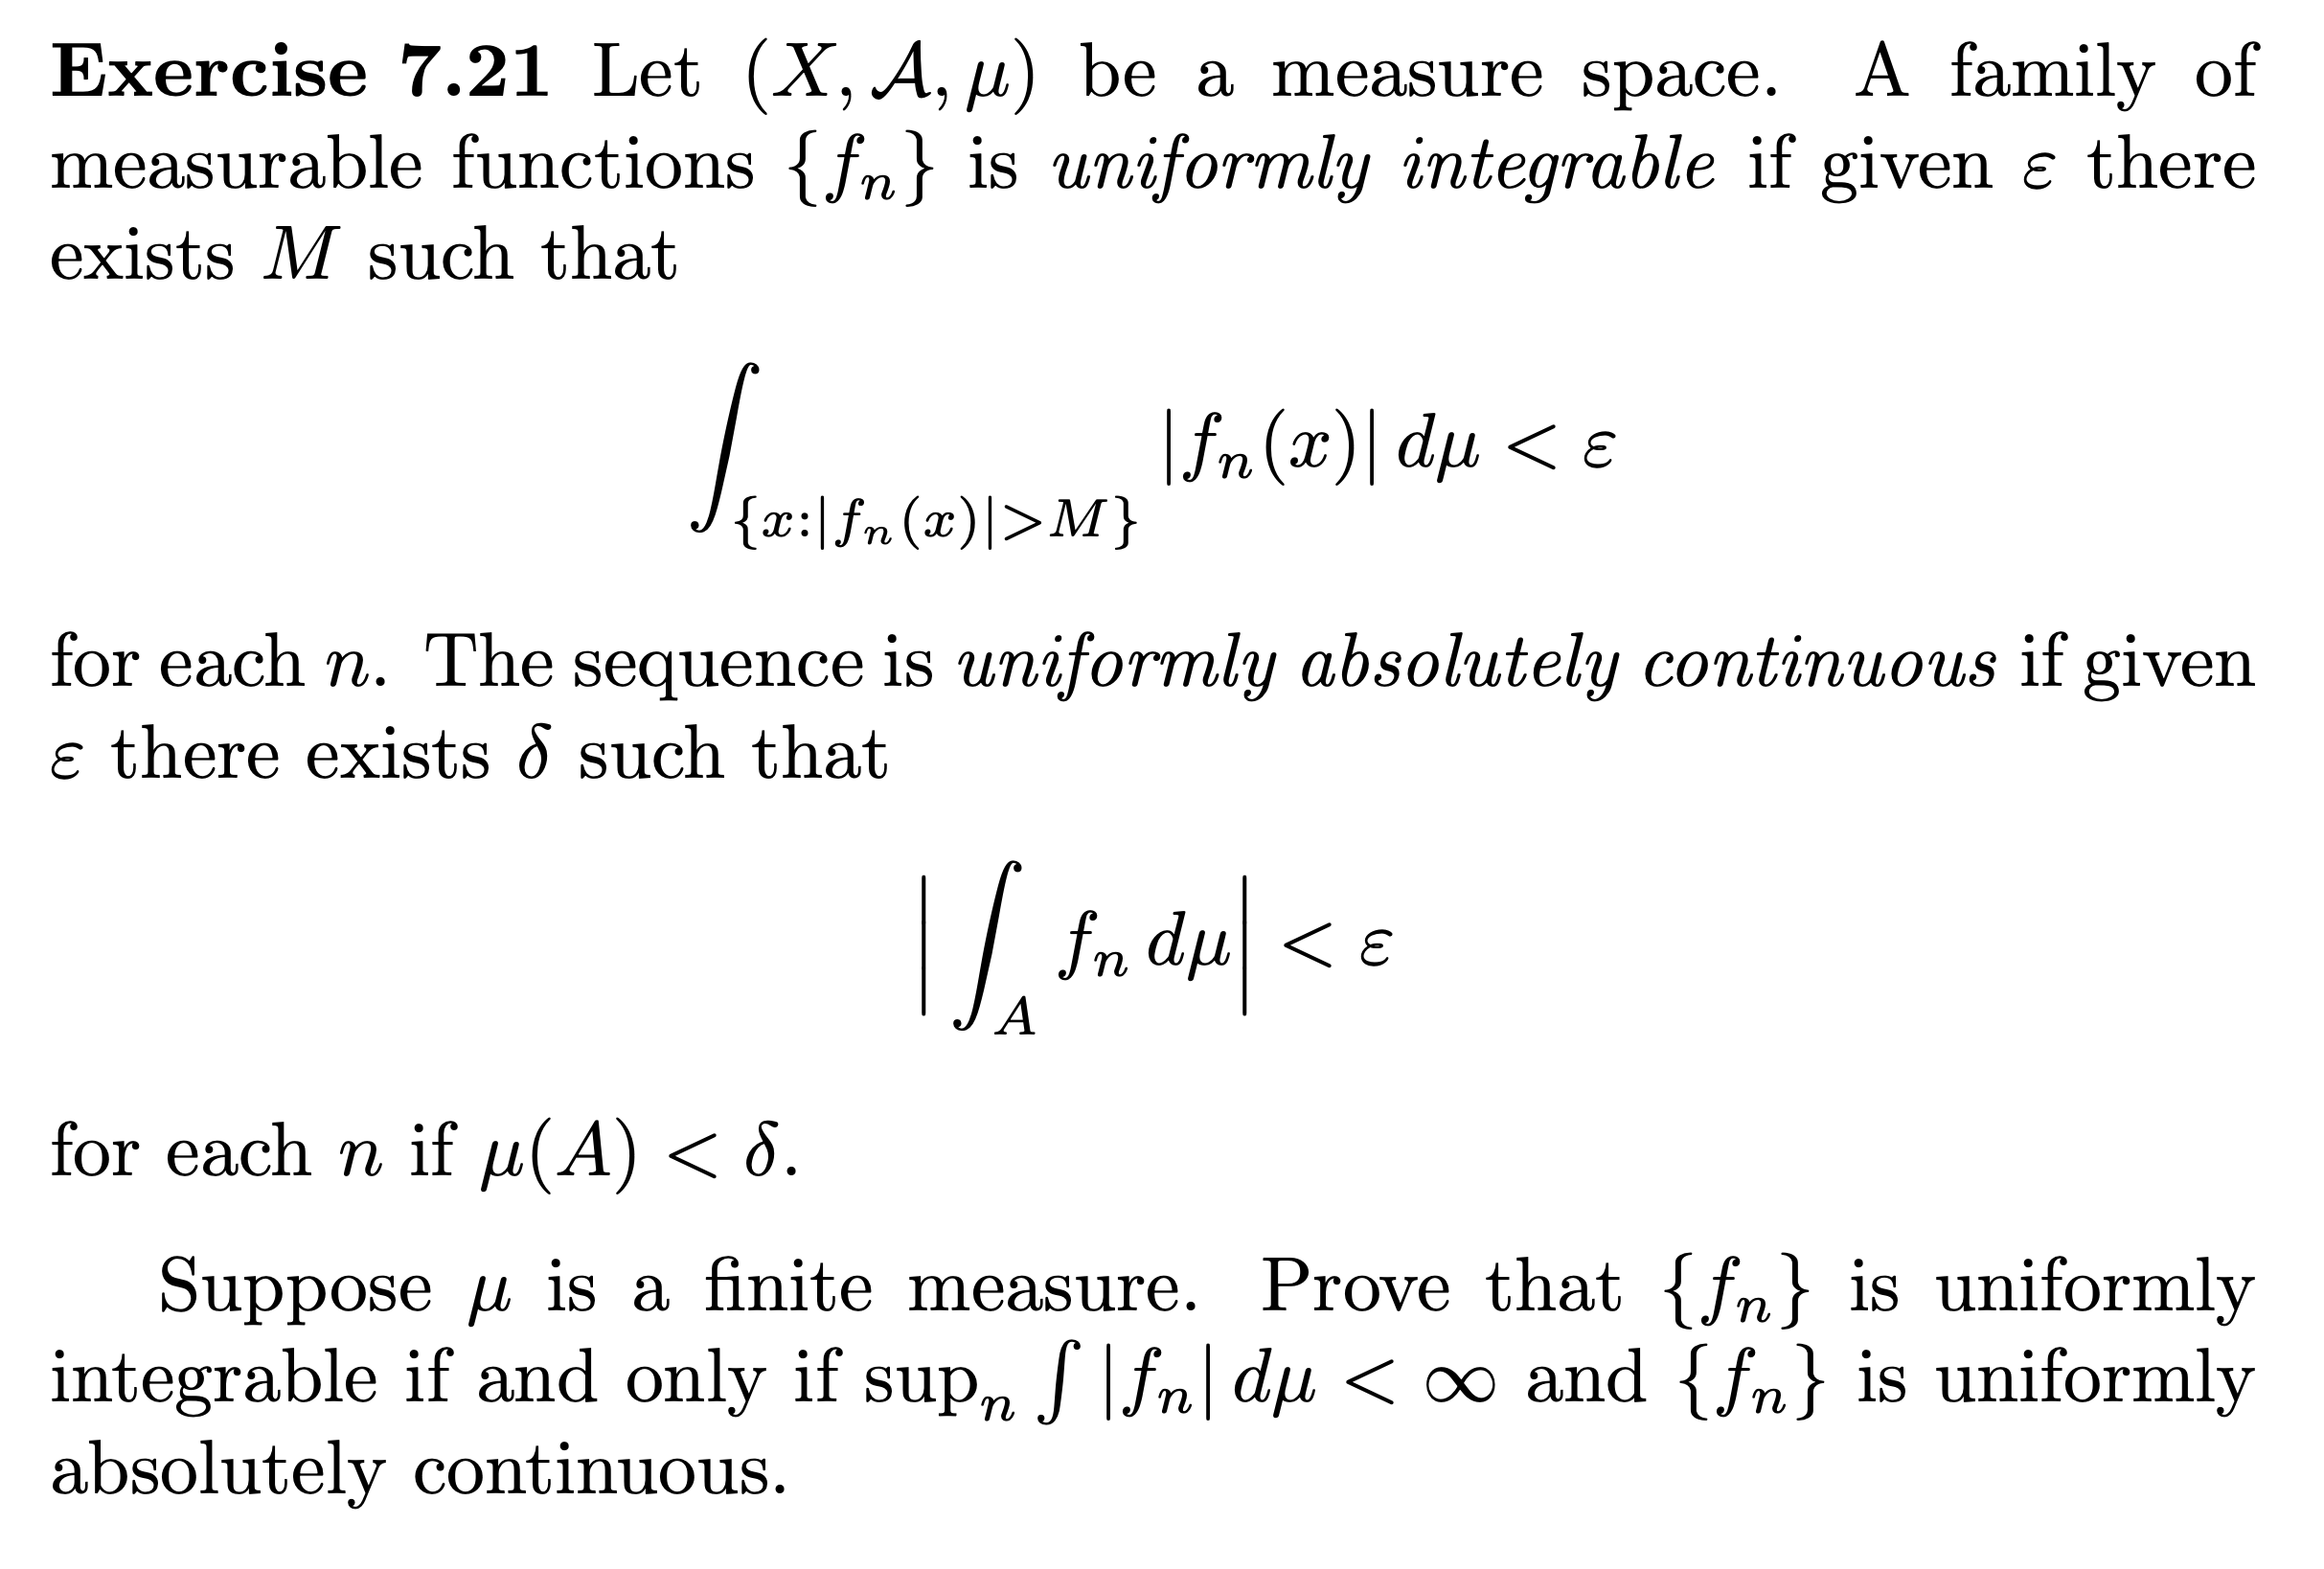
\includegraphics[width=400pt]{img/analysis--berkeley-202a-hw08-337f.png}
\end{mdframed}

\begin{intuition*}
  Saying that a sequence of functions $(f_n)$ is uniformly integrable is a bit like saying that, while they may
  be unbounded, they are integrable, and furthermore the control is uniform in the sense that the same $M$
  works for all $f_n$.

  Saying that a sequence of integrals is uniformly absolutely continuous is like saying that small changes in
  measure yield small changes in area, and furthermore that the control is uniform in the sense that the
  same $\delta$ works for all $f_n$.

  The supremum condition on the RHS is similar to saying that every $f_n$ is integrable, but stronger:
  the $f_n$ could be all integrable with the relevant sequence of integrals unbounded, but the given condition
  states that in addition to all being integrable, the sequence of integrals has an upper bound.

  So the reverse direction is a bit like saying that if (a) small changes in measure yield small changes in
  area, and (b) if the sequence of integrals is bounded above, then the functions are integrable.

  And the forwards direction is a bit like saying that if the functions are integrable (although possibly
  unbounded), then (a) small changes in measure yield small changes in area and (b) the sequence of integrals
  is bounded above.
\end{intuition*}

We break the proof into three separate claims (two for the forwards direction and one for the reverse direction).

\begin{claim*}
  If the $\{f_n\}$ are uniformly integrable then $\sup \int |f_n| < \infty$.
\end{claim*}

\begin{proof}
  Let $\eps > 0$ and let $M$ be such that for each $n$
  \begin{align*}
    \int_{\{x ~:~ |f_n(x)| > M\}} |f_n| < \eps.
  \end{align*}

  Let $U = \mu(X) < \infty$. Thus we have for each $n$
  \begin{align*}
    \int |f_n|
    &= \int_{\{x ~:~ |f_n(x)| > M\}} |f_n| + \int_{\{x ~:~ |f_n(x)| \leq M\}} |f_n| \\
    &< \eps +  M \mu\Big(\{x ~:~ |f_n(x)| \leq M\}\Big) \\
    &\leq \eps + MU.
  \end{align*}
  Hence $\eps + MU < \infty$ is an upper bound on $\int |f_n|$ and we have $\sup \int |f_n| < \infty$.
\end{proof}

\begin{claim*}
  If the $\{f_n\}$ are uniformly integrable then they are uniformly absolutely continuous.
\end{claim*}

\begin{proof}
  Let $\eps > 0$ and let $M$ be such that for each $n$
  \begin{align*}
    \int_{\{x ~:~ |f_n(x)| > M\}} |f_n| < \frac{\eps}{2}.
  \end{align*}
  Set $\delta = \frac{\eps}{2M}$ and let $A \in \mc A$ with $\mu(A) < \delta$.

  We have
  \begin{align*}
    \Bigg|\int_A f_n\Bigg|
    &< \int_A |f_n| \\
    &= \int_{\{x \in A ~:~ |f_n(x)| > M\}} + \int_{\{x \in A ~:~ |f_n(x)| \leq M\}} \\
    &< \frac{\eps}{2} + M\mu(A) \\
    &< \frac{\eps}{2} + M\frac{\eps}{2M} \\
    &= \eps,
  \end{align*}
  as required.
\end{proof}

\begin{claim*}
  If $\origsup_n \int |f_n| < \infty$ and the $\{f_n\}$ are uniformly absolutely continuous then they are
  uniformly integrable.
\end{claim*}

\begin{proof}
  Let $\eps > 0$.

  Let $B = \origsup_{n} \int |f_n|$ and let $\delta > 0$ be such that for all $n$ and all $A \in \mc A$
  if $\mu(A) < \delta$ then $\big|\int_A f_n\big| < \eps/2$.

  We want to show that there exists $M$ such that for all $n$
  \begin{align*}
    \int_{\{x ~:~ |f_n(x)| > M\}} |f_n| < \eps.
  \end{align*}
  Note that
  \begin{align*}
  \mu\big(\{x ~:~ f_n(x) > B/\delta\}\big) B/\delta < \int_{\{x ~:~ f_n(x) > B/\delta\}} f_n \leq B.
  \end{align*}
  Set $M = B/\delta$. Then
  \begin{align*}
    \mu\big(\{x ~:~ f_n(x) > M\}\big) < \delta,
  \end{align*}
  and therefore
  \begin{align*}
    \Bigg|\int_{\{x ~:~ f_n(x) > M\}} f_n\Bigg| = \int_{\{x ~:~ f_n(x) > M\}} f_n < \eps/2.
  \end{align*}
  Similarly
  \begin{align*}
    \mu\big(\{x ~:~ f_n(x) < -B/\delta\}\big) \cdot (-B/\delta) < \int_{\{x ~:~ f_n(x) < B/\delta\}} -f_n \leq B,
  \end{align*}
  and so
  \begin{align*}
    \mu\big(\{x ~:~ f_n(x) < -M\}\big) < \delta,
  \end{align*}
  hence
  \begin{align*}
    \Bigg|\int_{\{x ~:~ f_n(x) < -M\}} -f_n\Bigg| = \int_{\{x ~:~ f_n(x) < -M\}} -f_n < \eps/2.
  \end{align*}
  Therefore
  \begin{align*}
    \int_{\{x ~:~ |f_n(x)| > M\}} |f_n|
    &= \int_{\{x ~:~ f_n(x) > M\}} f_n + \int_{\{x ~:~ f_n(x) < -M\}} -f_n \\
    &< \frac{\eps}{2}+ \frac{\eps}{2} = \eps,
  \end{align*}
  as required.
\end{proof}